\section{Overbelægning}

\subsection{Udvikling og betydning af overbelægning}
Overbelægning opstår, når en afdeling har flere indlagte patienter end tilgængelige sengepladser. \citep{denstoredanskeordbog1} Hospitalsafdelinger med en belægningsprocent på over 85 estimeres til at have overbelægning. I perioden fra år 1996 til 2011 er sengepladserne på de danske hospitalsafdelinger reduceret med 30 \%, for således at opnå en fuld udnyttelse af ressoucerne. Herunder udnyttelse af de tilgængelige sengepladser på hospitalsafdelingerne samt optimering af sundhedspersonalets arbejdstid \citep{Madsen2014}. 


\subsection{Overbelægning i Danmark}
Antallet af indlagte patienter varierer hver måned, hvorfor tilgængeligheden af sengepladser ligeledes varierer. På \autoref{fig:overbelaegning_ran} er det illustreret, hvordan de forskellige afdelinger  på tværs af Danmark, oplever overbelægning i januar måned år 2015.

JEG ER KOMMET HER TIL!!!

\begin{figure}[H]
\centering
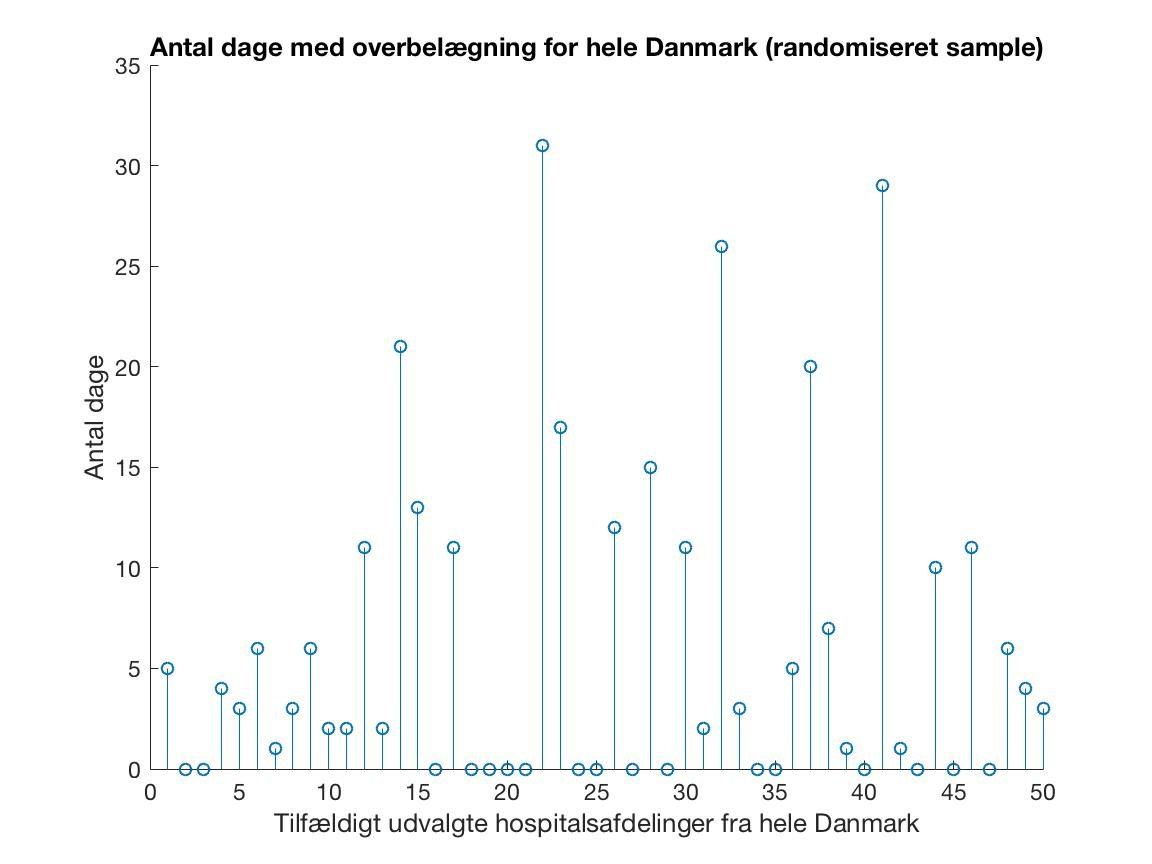
\includegraphics[width=1\textwidth]{figures/overbelaegning_ran.fig}
\caption{Antal dage med overbelægning udarbejdet med tilfældigt udvalgte hospitalsafdelinger fra hele Danmark. De randomiserede data er taget over januar måned i år 2015. \citep{SDS2015} \fxnote{uddyb figuren mere}} 
\label{fig:overbelaegning_ran}
\end{figure}

\noindent
Det ses af \autoref{fig:overbelaegning_ran}, at der er en tendens til overbelægning på flere hospitalsafdelinger i Danmark i forhold til underbelægning. Overbelægning strækker sig op til en måned. Det fremgår yderligere at der er en uligvægt mellem over- og underbelægning på de enkelte afdelinger. I de måneder hvor overbelægningen er størst, hvilket er januar til marts er overbelægningen på over 5 dage. Hvis der tages udgangspunkt i en enkelt afdeling understøttes det at der er et skel mellem over- og underbelægning.\citep{SDS2015} \fxnote{omskriv afsnit - det har ikke noget med underbelægning at gøre}

\begin{figure}[H]
\centering
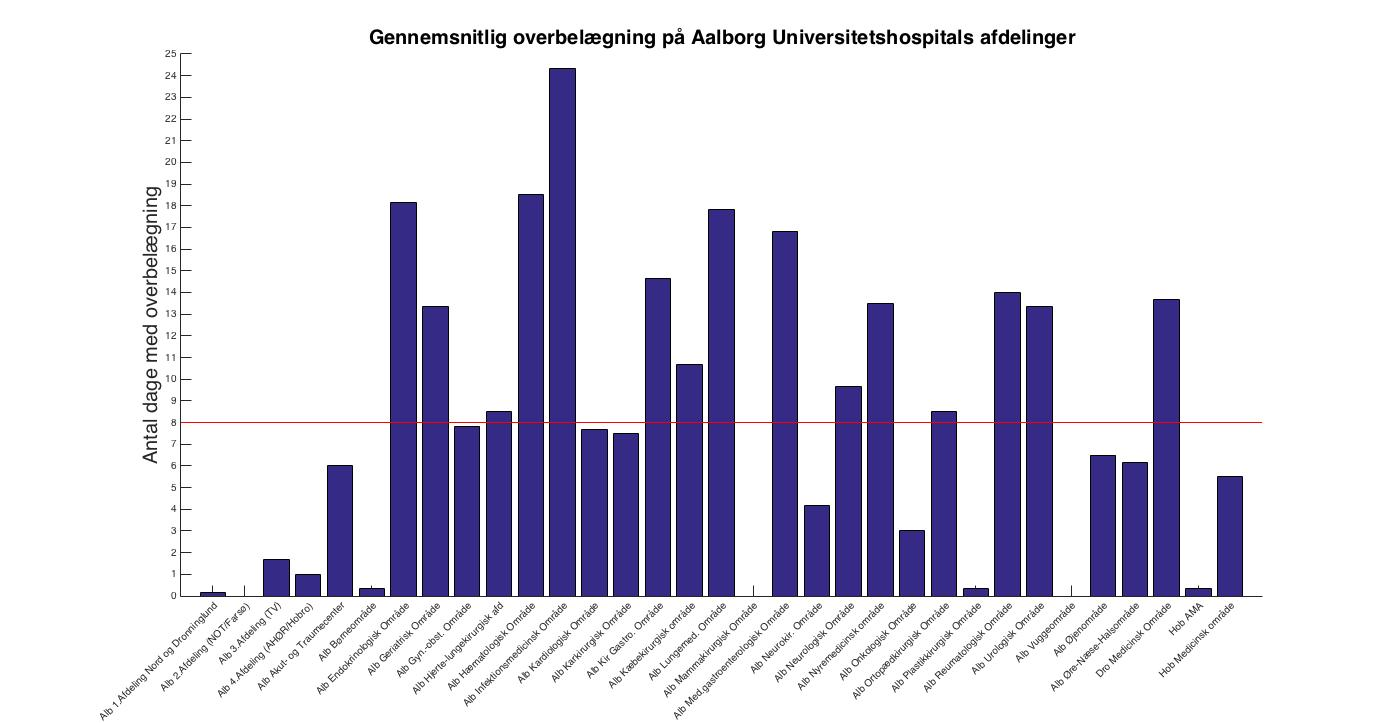
\includegraphics[width=1\textwidth]{figures/overbelaegning_AUH.fig}
\caption{Gennemsnitlig overbelægning på Aalborg Universitetshospitalsafdelinger målt i antal dage. Målingerne er taget for samtlige afdelinger på Aalborg Universitetshospital og er taget fra januar til juni i år 2015.\citep{SDS2015} \fxnote{omskriv og udddyb det med gennemsnit}}
\label{fig:overbelaegning_AUH}
\end{figure}

\noindent
Det fremgår af \autoref{fig:overbelaegning_AUH}, at den gennemsnitlige overbelægning på Aalborg Universitetshospital strækker sig op til 24 dage. \fxnote{skrives om ift grafen, nævn om forskellig grad. og nævn kun 1 søjle af overbelægning} Overbelægninger er størst på ambulatorisk infektionsmedicinsk område, ambulatorisk hæmatologisk område og ambulatorisk endokirinologisk. Det fremgår yderligere, at der ingen overbelægninger er på ambulatorisk 2. afdeling, ambulatorisk mammakirugisk  område og ambulatorisk vuggeområde. Det ses desuden, at den gennemsnitlige overbelægning på samtlige afdelinger varer op til 8 dage.\fxnote{omskrives} 

graf over stigende/faldende overbelægning over år. 




